% 
% Annual Cognitive Science Conference
% Sample LaTeX Paper -- Proceedings Format
% 

% Original : Ashwin Ram (ashwin@cc.gatech.edu)       04/01/1994
% Modified : Johanna Moore (jmoore@cs.pitt.edu)      03/17/1995
% Modified : David Noelle (noelle@ucsd.edu)          03/15/1996
% Modified : Pat Langley (langley@cs.stanford.edu)   01/26/1997
% Latex2e corrections by Ramin Charles Nakisa        01/28/1997 
% Modified : Tina Eliassi-Rad (eliassi@cs.wisc.edu)  01/31/1998
% Modified : Trisha Yannuzzi (trisha@ircs.upenn.edu) 12/28/1999 (in process)
% Modified : Mary Ellen Foster (M.E.Foster@ed.ac.uk) 12/11/2000
% Modified : Ken Forbus                              01/23/2004
% Modified : Eli M. Silk (esilk@pitt.edu)            05/24/2005
% Modified : Niels Taatgen (taatgen@cmu.edu)         10/24/2006
% Modified : David Noelle (dnoelle@ucmerced.edu)     11/19/2014
% Modified : Roger Levy (rplevy@mit.edu)     12/31/2018



%% Change "letterpaper" in the following line to "a4paper" if you must.

\documentclass[10pt,letterpaper]{article}

\usepackage{cogsci}
\usepackage{graphicx}

\cogscifinalcopy % Uncomment this line for the final submission 

\usepackage{pslatex}
\usepackage{apacite}
\usepackage{float} % Roger Levy added this and changed figure/table
                   % placement to [H] for conformity to Word template,
                   % though floating tables and figures to top is
                   % still generally recommended!



% NB: new command for "coursekata" shortening \ck
\newcommand{\ck}{\textit{CourseKata}}

\usepackage{xcolor}
\usepackage{soul}

\title{Linking student psychological orientation, engagement, and learning in college-level introductory data science}

\author{
    {\large{\textbf{Kristine Zheng (kxzheng@stanford.edu)\textsuperscript{1*}, Erik Brockbank\textsuperscript{1}, Shawn T. Schwartz\textsuperscript{1},}}} \\ 
    {\large{\textbf{David S. Yeager\textsuperscript{2}, Christopher Bryan\textsuperscript{2}, Carol Dweck\textsuperscript{1}, \& Judith E. Fan (jefan@stanford.edu)\textsuperscript{1}}}} \\
    \textsuperscript{1}Stanford University, USA \\ 
    \textsuperscript{2}University of Texas at Austin, USA 
}

\begin{document}

\maketitle


\begin{abstract}
Introductory data science courses have the potential to provide students from diverse backgrounds skills for working with and reasoning about data.
However, what predicts success in these courses remains poorly understood.
Here we investigate how students' initial psychological orientation relates to their subsequent engagement and learning.
In Study 1, we took an observational approach, analyzing data from 1306 students across 11 institutions using an interactive online textbook.
Students' psychological orientation, (e.g., math anxiety, stress expectations) predicted performance on assessments administered throughout the term.
In Study 2, we developed and tested an intervention targeting these aspects of students' learning experience among 146 students enrolled in a single course.
Preliminary analyses suggest that this intervention shifted students' beliefs about the relationship between stress and learning.
Taken together, this work contributes to our understanding of how affective and cognitive processes interact in real-world educational settings.

\textbf{Keywords:} 
education; mindset; field experiments; statistics, learning technology

\end{abstract}


% \section{Introduction} 

Formal tools for understanding data are vital for making sense of the modern world, especially phenomena that are too large, slow, or complex for people to observe directly (e.g., climate change, macroeconomic dynamics).
As such, data literacy has become indispensable for guiding evidence-based decision making both at the individual level (e.g., healthcare, financial planning) and at the societal level \cite{gal2002adults,provost2013data,muhammad2020predictive}. 
Understandably, then, data science curricula have undergone rapid development and expansion in recent years \cite{de2017curriculum, manyika2011big}.
Here we ask: What are the psychological factors that impact how well students acquire foundational data literacy skills in these learning environments?

%%% FIGURE: CourseKata dataset overview %%%
\begin{figure*}[htbp!]
\begin{center}
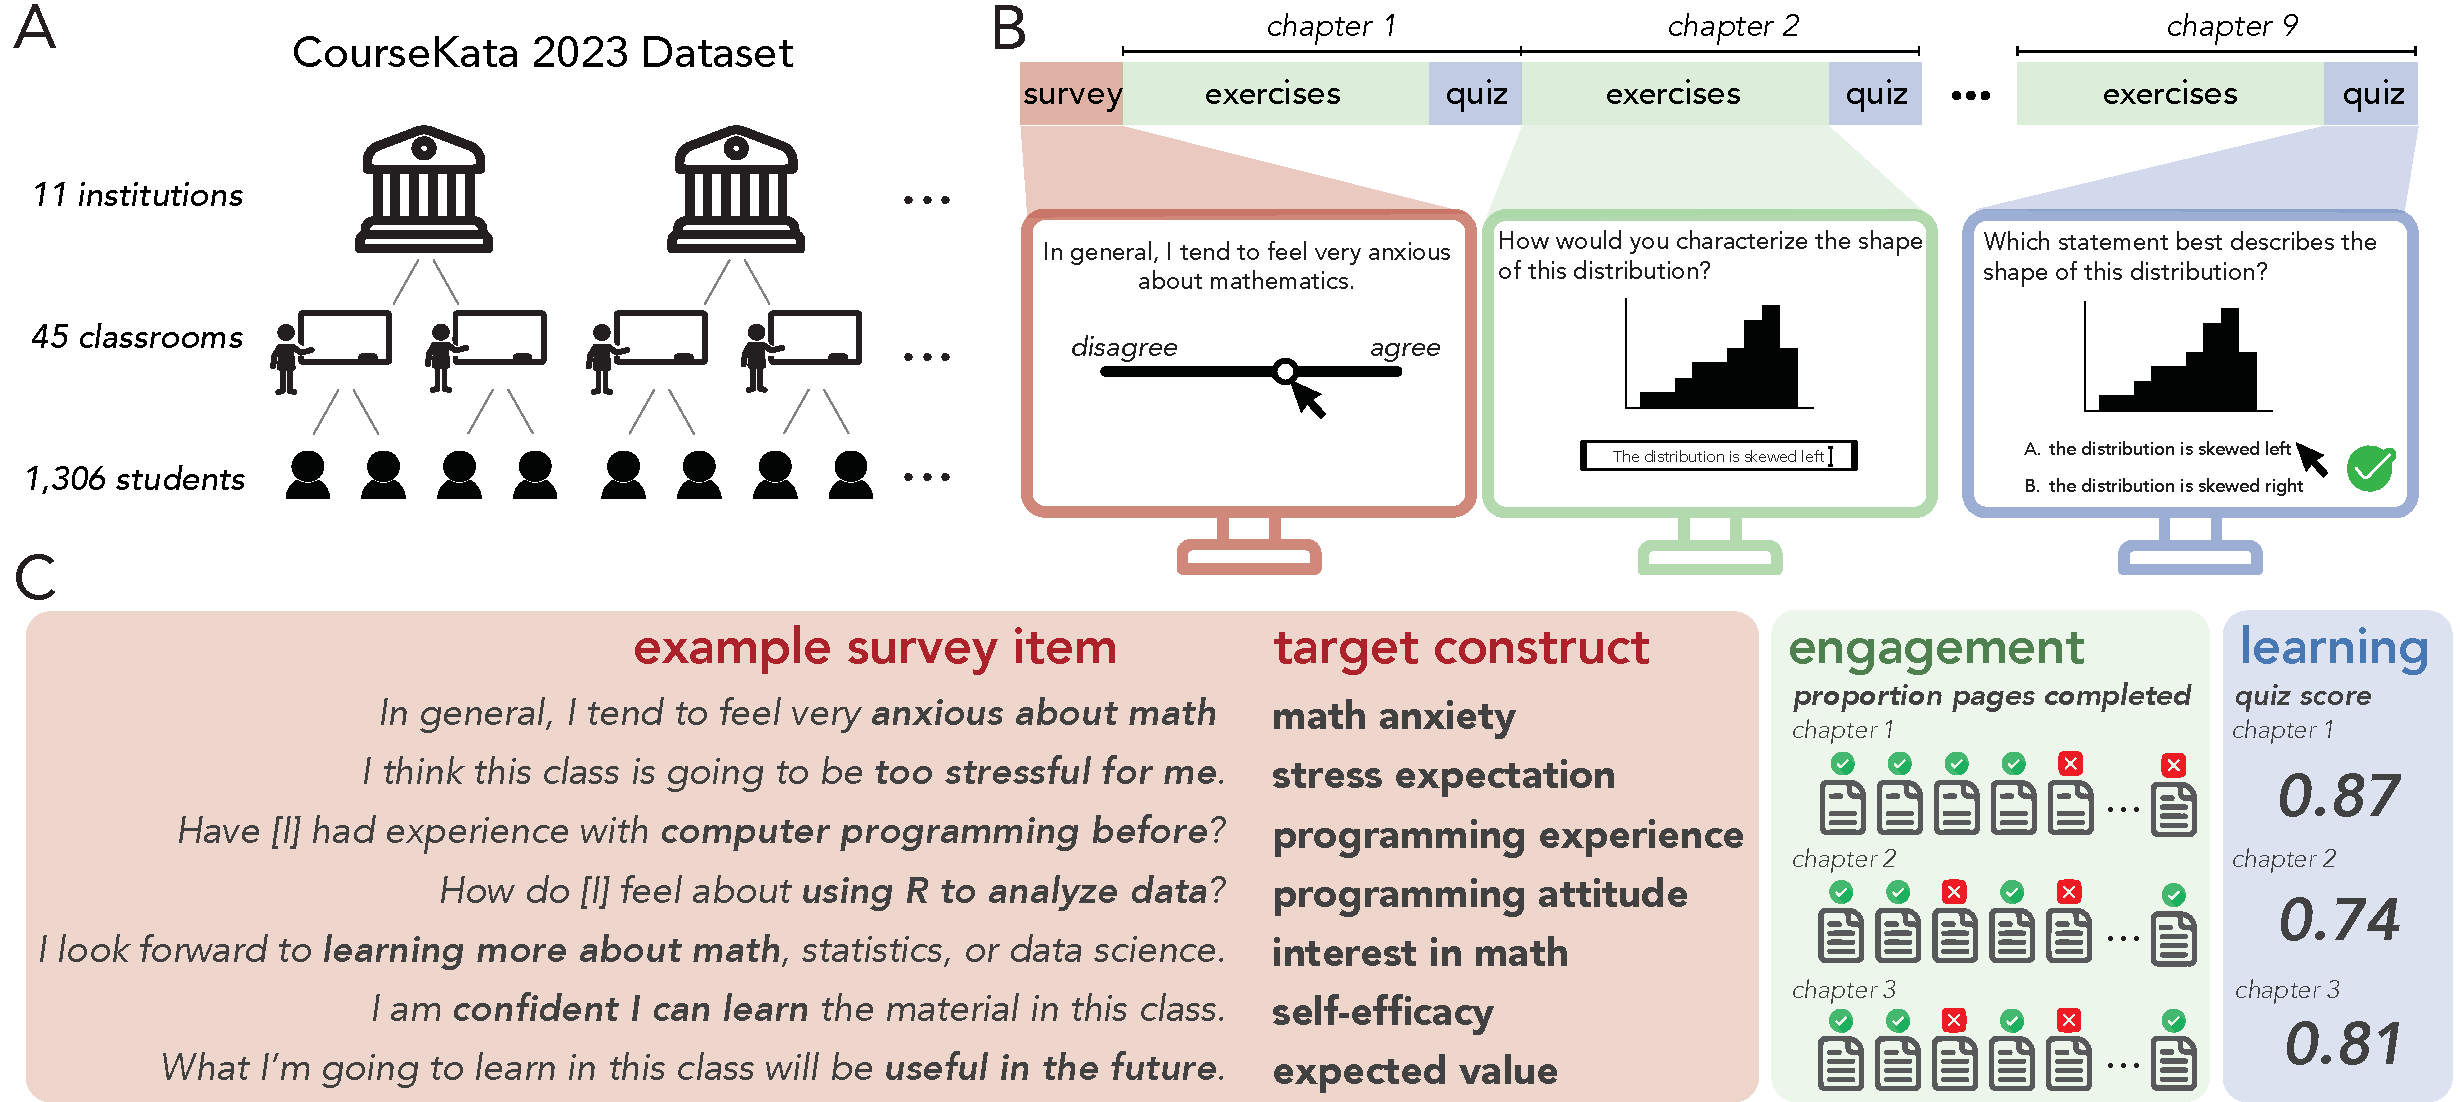
\includegraphics[width=0.95\linewidth]{figures_cogsci/ck_dataset_observation_methods_combined.pdf}
\end{center}
\caption{(A) Data from $1306$ students enrolled in $45$ courses across $11$ institutions were analyzed in the current study. 
(B) A digital textbook (\ck) was used to obtain survey-based measures of students' psychological orientation, as well as measures of engagement with learning activities and performance on end-of-chapter quizzes. 
(C) Example survey items used to measure seven aspects of initial student psychological orientation. Engagement was measured as the proportion of ``pages'' completed in each \ck{} chapter.} 
\label{fig:coursekata_content}
\end{figure*}

A wide array of factors, collectively contributing to a student's mindset, might influence how much and how well students learn in a data science course, including their goals, interests, motivations, attitudes, sense of belonging, and beliefs about themselves and the material \cite{dweck2017needs, murphy2007signaling, duckworth2007grit, bandura2001self, walton2007question, onwuegbuzie2003statistics}.
Prior work has found, for example, that the degree to which students adopt a growth mindset---the belief that their intellectual abilities are malleable---is meaningfully predictive of their ability to persist and succeed in challenging STEM subjects \cite{yeager2019national, yeager2020can, yeager2022synergistic}. 
Students' "strategic mindset" orientation---associated with metacognitive strategy use in goal pursuit---was indirectly predictive of progress towards challenging and long-term goals \cite{Chen2020strategic}.
Moreover, previous studies have investigated the degree to which students who are initially more apprehensive about the course, such as by having higher levels of test anxiety or by being less confident they will succeed, perform less well than other, less apprehensive students \cite{sutter2024concerns, zeidner2007test, cassady2002cognitive}. 

Similarly, prior work suggests that students who consider a course to be interesting and relevant to their long-term goals tend to be more engaged and to perform better than students who are less invested in the course \cite{hulleman2009promoting, harackiewicz2016interest}. 

However, the intrinsic complexity and heterogeneity in learning environments poses challenges for understanding the relationship between these psychological factors and student learning outcomes \cite{brown1992design}. 
Detailed measurement of student beliefs and behavior across a wide range of learning conditions are critical for beginning to meet this challenge \cite{bryan2021behavioural}.
Newly developed digital learning environments make it possible to track student learning behavior over time in larger and more diverse populations of learners \cite{reza2021mooclet, stigler2020better, motz2018embedding, lovett2008jime}.
These larger longitudinal datasets make it feasible to develop quantitative models that account for more complex interactions between sources of variation across individuals and groups.

% Current work
Here we leverage longitudinal data obtained using one such digital learning platform, \ck{} \cite{stigler2020better}, to explore links between student psychological orientation and subsequent engagement \cite{gao2025predicting, henrie2015measuring} and learning behavior. 
We begin with an observational approach by analyzing sources of variation in learning among 1306 students enrolled in college-level introductory data science courses across 45 classrooms in 11 institutions.
Based on insights from that study, we then explored the potential for an intervention targeting students' appraisal of stress and their tendency to seek alternative strategies when stuck.
In an initial study with one university course, we measured the impact of this intervention on students' subsequent psychological orientation towards the course \cite{yeager2022synergistic, Chen2020strategic}.
By combining insights from large observational datasets with targeted experimental interventions, the current work contributes to our understanding of learning in real-world educational environments. 

\section{Study~1: Characterizing the relationship between student psychological orientation and learning}

We first sought to understand the aspects of students' psychological orientation that predict engagement and learning dynamics in introductory data science courses.
Towards this end, we leveraged publicly available data collected using a digital textbook known as \ck{} \cite{stigler2020better}.

\subsection{Methods}
\paragraph{Participants}
Our study analyzed data from 1306 college students (\textit{gender}:  $72.82\%$ female, $24.66\%$ male, $1.91\%$ non-binary, and $0.61\%$ undisclosed; \textit{race}: $36.06\%$ Latine, $24.27\%$ Asian, $22.13\%$ White, $5.51\%$ Black, $3.98\%$ Middle Eastern, $0.46\%$ American Indian or Alaska Native, $0.31\%$ Native Hawaiian or Pacific Islander, $7.38\%$ undisclosed) who enrolled in 45 unique data science courses across 11 institutions (Fig.~\ref{fig:coursekata_content}A). 
Only data from students who provided consent for their data to be used in educational research were included and their data were anonymized in accordance with the University of California, Los Angeles IRB. Note that because textbook activities, particularly surveys, were optional for students, modeling analyses focus on a subset of all the students in the dataset.

\noindent \textbf{\ck{}-2023 Dataset}
The \ck{} textbook contains 12 chapters covering core concepts in statistics and how to construct statistical models to explain variation in quantitative data \cite{son2021modeling}. Data from the first nine chapters were available for analysis. 
Students first completed a pre-course survey of prior experience and attitudes toward the material. 
The subsequent chapters included interleaved content and learning activities which combined questions probing conceptual understanding with exercises using the R programming language. 
Student learning was assessed with a quiz at the end of each chapter (Fig.~\ref{fig:coursekata_content}B). 


\noindent \textbf{\textit{Psychological orientation}}
Various aspects of students' psychological orientation were measured using 6-point Likert-scale responses to survey items embedded in the opening section of the textbook.
Our study focuses on survey items targeting seven constructs: math anxiety, stress expectation, prior programming experience, attitude towards programming, interest in math, self-efficacy, and the long-term expected value of the course material (Fig.~\ref{fig:coursekata_content}C). 
For constructs that were measured using multiple survey items, we computed the mean response across the items to derive a single estimate for that construct, for each student.
We used the mappings between individual survey items and target constructs that were defined by the \ck{} developers.

%%% FIGURE: Survey construct correlation matrix %%%
\begin{figure}[ht!]
\begin{center}
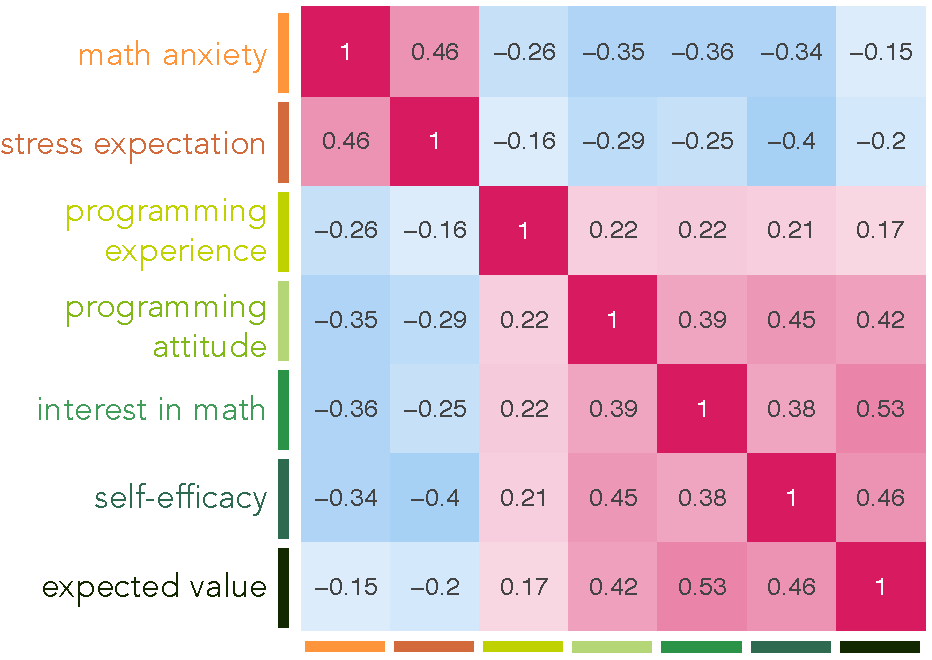
\includegraphics[width=0.9\linewidth]{figures_cogsci/observational_correlation_constructs.pdf}
\end{center}
 \caption{Pairwise comparisons of psychological construct ratings from initial \ck{} survey. Higher values indicate greater strength of associations between constructs. For all estimated correlation coefficents, $p< .001$.} 
\label{fig:coursekata_construct_clusters}
\end{figure}

\noindent \textbf{\textit{Learning}}
Student learning was measured at multiple time points throughout each course using the nine quizzes embedded at the end of chapters in \ck. 
These quizzes consisted of 12-32 multiple-choice questions that focused on the learning objectives for that chapter. 
We use average performance across end-of-chapter quizzes as a measure of each student's overall comprehension (Fig.~\ref{fig:summary}C).

\noindent \textbf{\textit{Engagement}}
Student engagement with the material was measured by tracking completion of interactive learning activities embedded in multiple ``pages'' throughout each chapter.
We estimated a student's \textit{level of engagement} by computing the proportion of pages a student completed from that chapter out of the maximum number of pages in the chapter completed by any student enrolled in the same course (Fig.~\ref{fig:summary}C).  
We consider a page to have been completed only if the student completed \textit{all} embedded learning activities on that page. 


\subsection{Results}

\paragraph{Understanding associations between various components of students' psychological orientation}

While we initially identified seven psychological constructs to focus on in the survey data ($N=1306$), we anticipated that these constructs might be associated with one another.
We estimated the strength of the associations by computing the Pearson correlation coefficient for every pair of constructs (Fig.~\ref{fig:coursekata_construct_clusters}). 
For each set of $k$ clusters, we calculated the corresponding \textit{silhouette score}---a measure of clustering strength that quantifies how closely items within a cluster are grouped relative to the distance between clusters \cite{shahapure2020cluster, rousseeuw1987silhouettes}. 
Using the correlation between constructs within and across clusters as a distance metric, we obtained a maximum silhouette score with $k=2$ clusters.
The resulting associated constructs included one group composed of \textit{math anxiety} and \textit{stress expectation}, while another consisted of \textit{prior programming experience}, \textit{attitude towards programming}, \textit{interest in math}, \textit{self-efficacy}, and the \textit{expected value} of the course in the long term. 
This grouping suggests reliable low-dimensional structure in these survey responses, thereby constraining how independently the seven constructs might contribute to predicting variation in subsequent learning. 

\paragraph{Relating student psychological orientation and engagement}
Given the potential for fluctuations in students' level of engagement throughout the course, we first assessed the reliability of our engagement metric in the \ck{} dataset.
To estimate reliability, individual textbook ``pages'' were assigned to two split halves of the textbook; each student's engagement score for each split half was the proportion of pages they completed in each split. 
We calculated the pairwise correlation between students' split-half engagement levels, corrected using the Spearman-Brown Formula.
This process was repeated to estimate uncertainty in the split-half reliability.
Overall, split-half reliability was high ($0.979$; bootstrapped 95\% CI $=[0.975, 0.982]$), suggesting that students' level of engagement was relatively consistent throughout the course. 

How well can variation \textit{between} students ($N=1209$) in overall engagement level be accounted for by differences in their psychological orientation? 
We fit a linear mixed-effects model estimating each student's average chapter-level engagement with the psychological constructs from the pre-course survey, while accounting for variation in engagement across individual students within each class. 
Students' survey responses across the psychological constructs of interest were not significant predictors of overall engagement ($\chi^2(7)=6.52$, $p=.48$).
This finding was not a result of the observed correlation between psychological constructs (Fig.~\ref{fig:coursekata_construct_clusters}); none of the psychological constructs \textit{individually} accounted for significant variation in overall engagement (\textit{math anxiety}: $\chi^2(1)=0.027$, $p=.87$; \textit{stress expectation}: $\chi^2(1)=0.38$, $p=.54$; \textit{self-efficacy}: $\chi^2(1)<0.001$, $p=.99$; \textit{programming attitude}: $\chi^2(1)=0.07$, $p=.80$; \textit{math interest}: $\chi^2(1)=0.03$, $p=.87$; \textit{expected value}: $\chi^2(1)=2.53$, $p=.11$; \textit{programming experience}: $\chi^2(1)=0.88$, $p=.35$).
Broadly, variation between students in their attitudes toward the material did not meaningfully predict differences in the proportion of interleaved activities they completed throughout each course.

\paragraph{Relating student psychological orientation, engagement, and learning outcomes}

In the preceding results, we found that students' level of engagement was relatively stable throughout the course and variation in psychological orientation did not account for individual variation in engagement.
How might both students' psychological orientation and engagement relate to learning, as measured by scores on end-of-chapter quizzes?
We fit a linear mixed-effects model estimating participants' average end-of-chapter quiz score with their engagement level and pre-course survey responses, while accounting for random variation in student performance within each class ($N=1209$). 

Overall, students' pre-course survey responses were a significant predictor of average quiz performance ($\chi^2(7)=40.04$, $p<.0001$). 
However, we did not find evidence for a relationship between this measure of engagement and quiz performance ($\chi^2(1)=2.59$, $p=.11$). 
Further, including students' level of engagement did not meaningfully improve the observed relationship between psychological orientation and quiz performance ($\chi^2(1)=2.05$, $p=.15$). 

Given the strong relationship between pre-course survey responses and quiz performance, we next investigated the degree to which this effect can be attributed to each group of survey constructs suggested by $k$-means clustering (Fig.~\ref{fig:coursekata_construct_clusters}).
We fit linear mixed-effects models to students' average quiz performance with the survey constructs in each cluster as predictors.
We compared models using the \textit{Akaike Information Criterion} (AIC), a standard measure of model fit that rewards models that explain the data better while penalizing additional parameters \cite{akaike1974new}.

We found that the combination of \textit{programming experience}, \textit{programming attitude}, \textit{interest in math}, \textit{self-efficacy}, and \textit{expected value} of the course predicted individual variability in quiz performance beyond what can be attributed to random variation among students within each class (relative AIC $=-14.20$; Fig.~\ref{fig:coursekata_eoc_survey_aic}). %avg relative AIC $=-13.77$%
In addition, \textit{math anxiety} and \textit{stress expectation} alone were comparably strong predictors of quiz performance (relative AIC $=-15.28$). %avg rel AIC = $=-17.54$%
Finally, a \textit{full model} with all seven pre-course survey constructs outperformed each individual group of constructs (relative AIC $=-26.04$). %  %avg rel AIC = $=-29.43$% 
These results suggest that students' psychological orientation towards the course were important predictors of learning outcomes.

%%% FIGURE: engagement and quiz dyanamics thoughout course %%%
\begin{figure}[t]
\centering    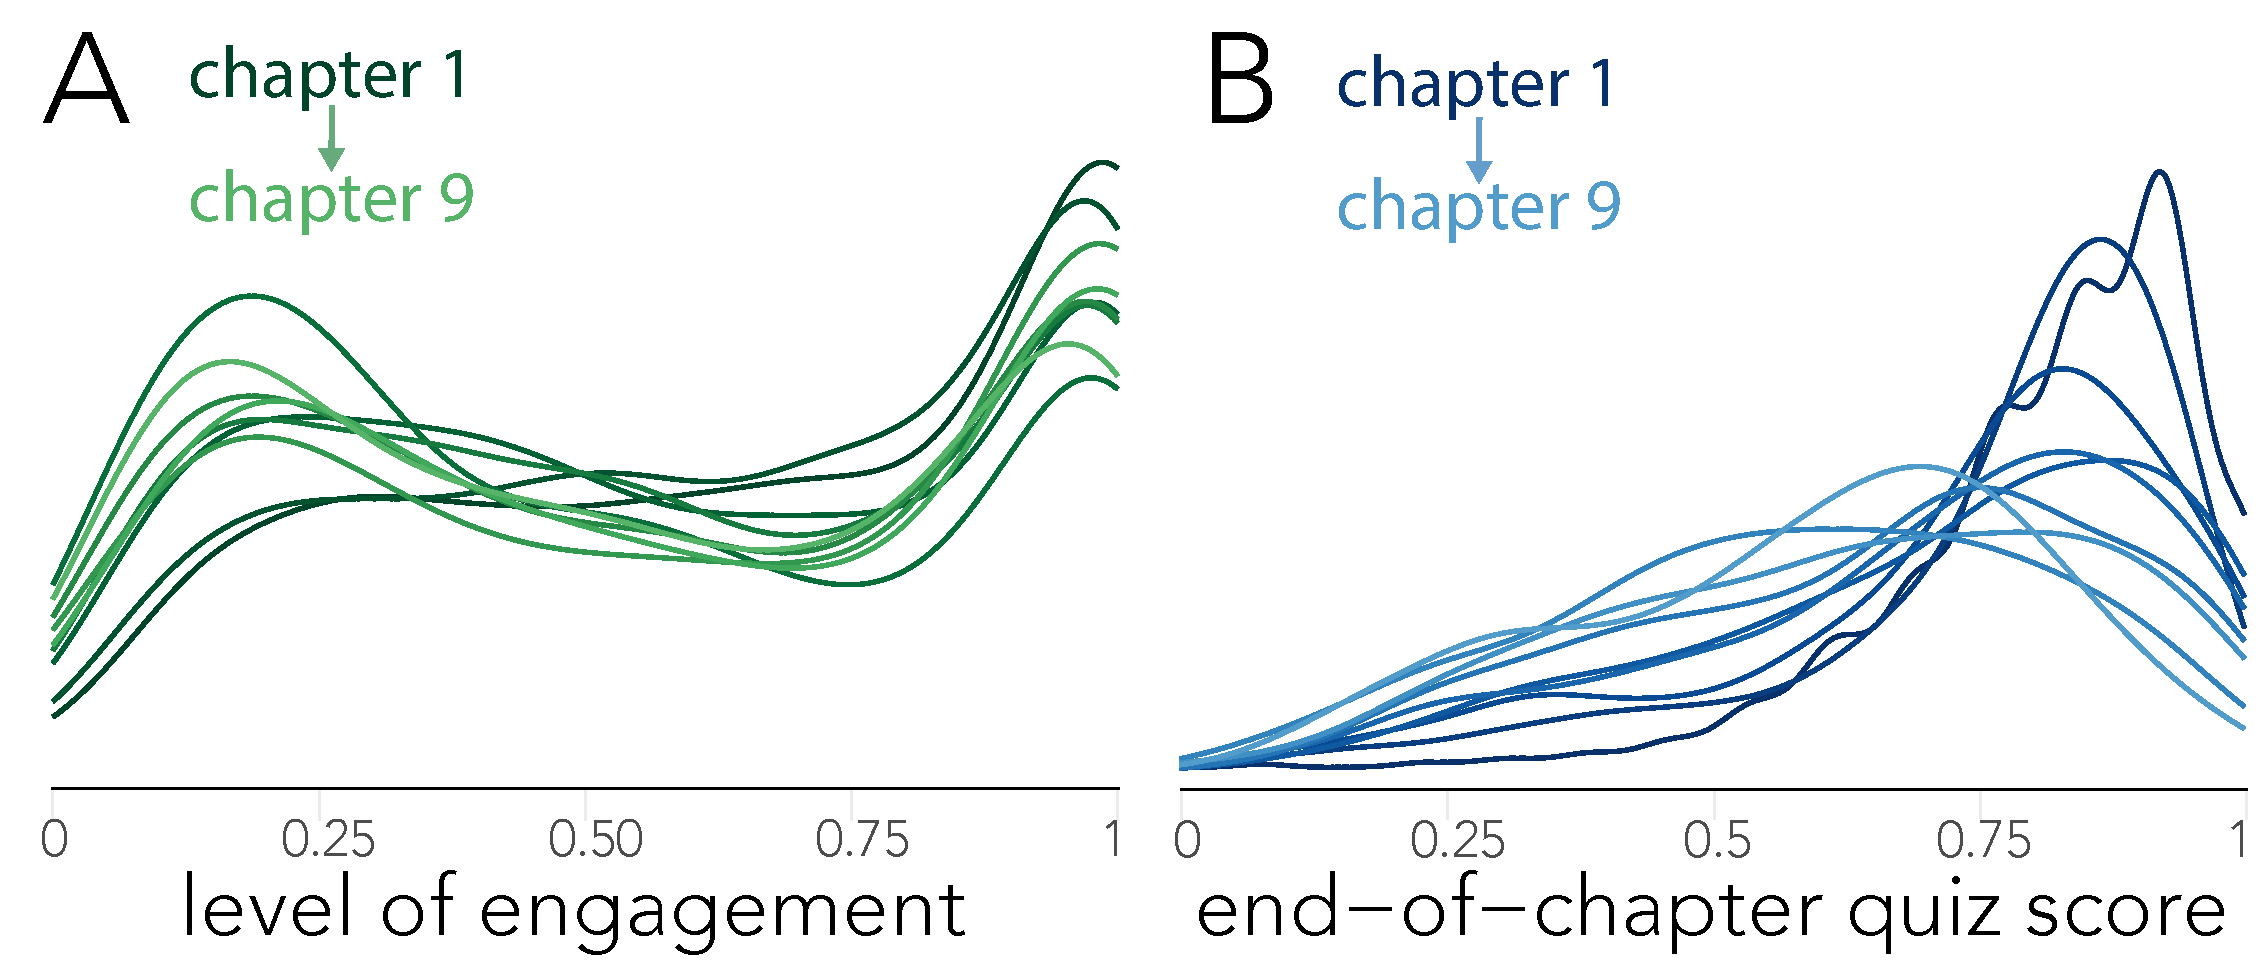
\includegraphics[width=0.99\linewidth]{figures_cogsci/2023_coursekata_kde_chapters_distribution.pdf}
    \caption{(A) Distribution of page completion rates for interleaved activities for each chapter in \ck{} (plotted with kernel density estimation). 
    (B) Distribution of performance on end-of-chapter quizzes for each chapter in \ck{} (plotted with kernel density estimation).}
    \label{fig:summary}
\end{figure}


%%% FIGURE: Study~1 model comparison %%%
\begin{figure}[th!]
\begin{center}
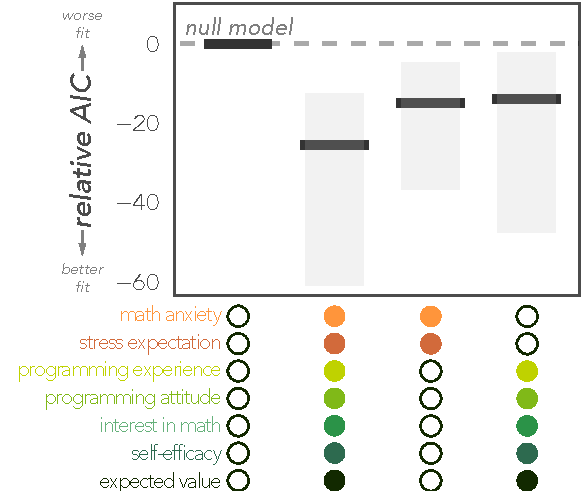
\includegraphics[width=0.85\linewidth]{figures_cogsci/2023_student_eoc_construct_aic.pdf}
\end{center}
\caption{Comparison between models predicting performance on interleaved assessments from various survey-based measures of students' psychological orientation. The inclusion of a predictor in a model is indicated by the filled colored discs. The position of each dark horizontal bar indicates the relative improvement in model fit, measured using AIC, relative to the null model (dashed line). Light gray rectangles represent the expected range of values for the models' relative AIC due to sampling variation, estimated via bootstrap resampling of students within each class.} 
\label{fig:coursekata_eoc_survey_aic}
\end{figure}

\section{Study 2: Impact of a mindset intervention on student psychological orientation}

In Study~1, we found that students' psychological orientation at the start of the course was reliably associated with subsequent quiz performance. 
As a next step, we sought to take initial steps towards developing interventions that might shift students' mindsets about stress and their metacognitive awareness when working through problems, which might play a role in improving students' learning experiences and outcomes.

Adapting interventions developed in previous work, our intervention focused on two dimensions of students' learning experiences in introductory data science courses.

First, this intervention aimed to help students understand that stress can be useful (a \textit{stress-can-be enhancing} mindset). That is, they were taught to reframe moderate levels of stress and frustration (e.g., frustration with computer programming) as opportunities for learning and growth \cite{yeager2022synergistic, crum2013rethinking}. 
Second, it highlighted a “strategic mindset,” that is, the value of metacognitive awareness as to whether, when working through a difficult problem, it might be worthwhile to seek alternative approaches \cite{Chen2020strategic}. 
Here we report initial insights from measuring the impact of this intervention on these two dimensions in a single data science course.

\subsection{Methods}
%%% Figure: Study~2 experiment setup and results %%%
\begin{figure*}[t]
\begin{center}
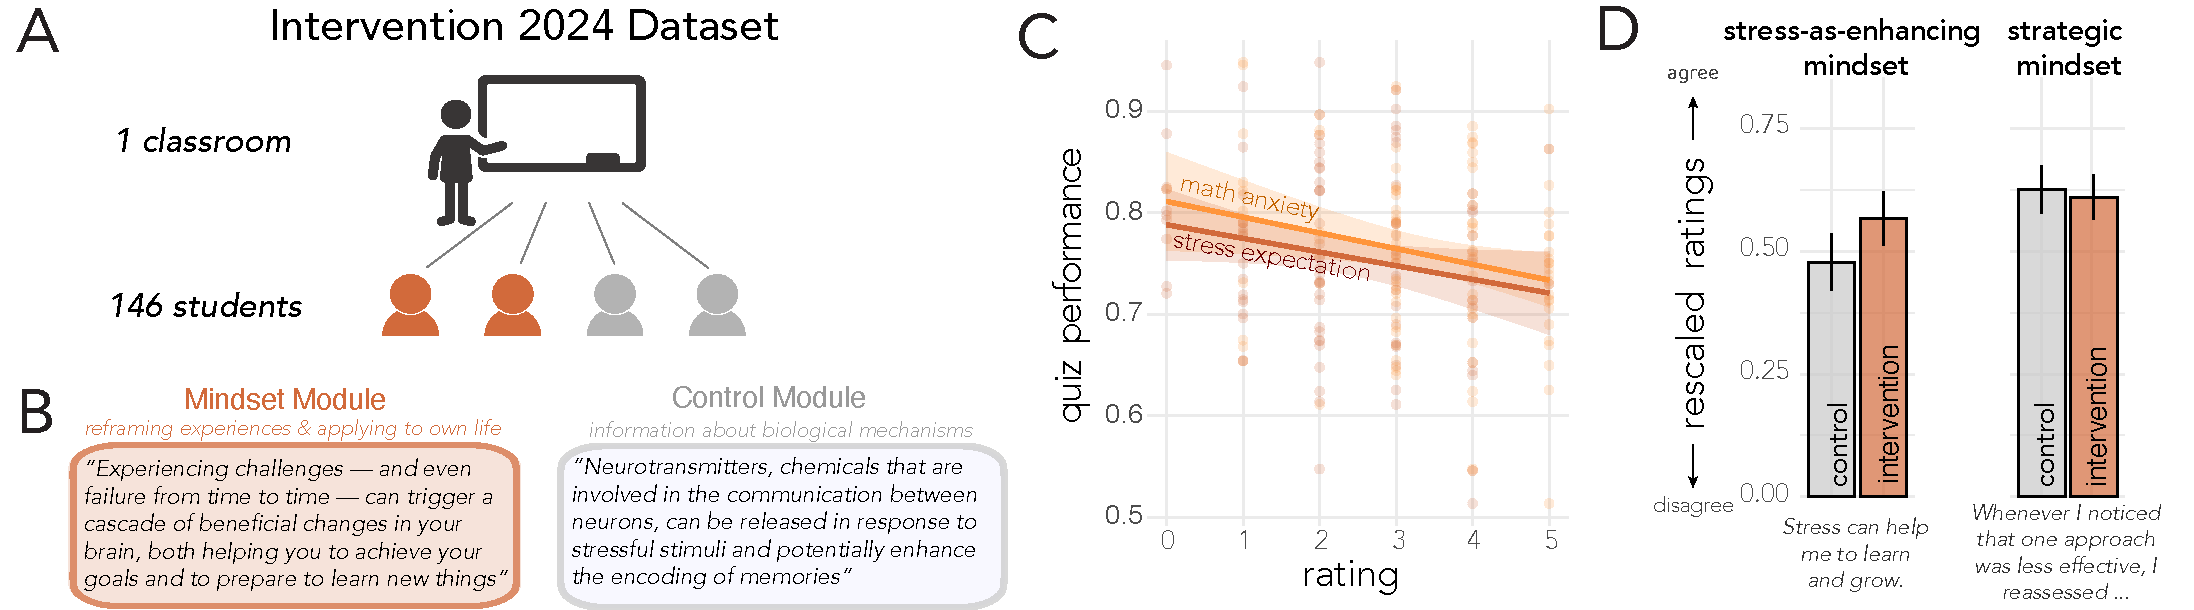
\includegraphics[width=0.99\linewidth]{figures_cogsci/2024_experimental_methods_results_combined.pdf}
\end{center}
\caption{
(A) Students ($N=146$) were randomly assigned to either the mindset intervention and control condition. 
(B) The mindset condition provided students with specific strategies for reframing stressful experiences in the classroom as opportunities to learn and grow, and for understanding the importance of a strategic mindset. The control condition provided an overview of key concepts in neuroscience related to the phenomenon of learning and stress, but no guidance as to how to apply those concepts to their experiences as students.
(C) Associations between quiz performance and students' initial math anxiety and expectations about how stressful the course would be.
(D) Student mindsets about stress and metacognitive awareness while learning following the intervention. %``Stress-as-enhancing" mindset was reliably different between two intervention conditions.
}
\label{fig:intervention-experiment-flow}
\end{figure*}

\paragraph{Participants}
Data was collected from 146 students (\textit{gender}: $69.18\%$ female, $24.66\%$ male, and $6.16\%$ nonbinary; 
\textit{race}: $23.97\%$ White, $23.29\%$ Asian, $17.81\%$ Latine, $14.38\%$ Black, $4.79\%$ Middle Eastern, $2.05\%$ American Indian or Alaska Native, $12.33\%$ Multiracial, and $1.37\%$ undisclosed) enrolled in a college-level introductory data science course using the \ck{} platform in Fall 2024 at Stanford University (Fig.~\ref{fig:intervention-experiment-flow}A). 
Students provided consent for their data to be used in research (7 students who opted out of the study are not included in the analyses). 
Participant data is anonymized in accordance with the Stanford University IRB. 
Note that because study activities, particularly surveys, were optional for students in accordance with the IRB protocol, different analyses focus on different subsets of the full classroom dataset.


\noindent \textbf{\textit{Psychological orientation}}
% \paragraph{Psychological orientation}
At the start of the term, students completed the \ck{} pre-course survey. 
The survey format and associated psychological constructs were identical to those described in Study~1. 
Survey items related to programming experience and programming attitudes were not included in these analyses due to a high number of missing responses.

\noindent \textbf{\textit{Mindset intervention}}
% \paragraph{Mindset intervention}
In the sixth week of the term (out of ten weeks), students completed a special module in class lasting approximately 30 minutes.
This module was administered in the second half of the term, rather than at the beginning, due to scheduling constraints independent of the design of this study.

Half of the students were randomly assigned to the mindset intervention condition, and this module helped students: (1) reframe stressful and challenging experiences in the classroom as opportunities to learn and grow and (2) to be aware of opportunities to seek alternative approaches when working through a difficult problem (e.g., writing code to analyze data). 
The other half of the class was provided with a \textit{control} module that introduced core concepts in neuroscience as they relate to learning and the experience of stress (e.g., \textit{plasticity}), but did not provide guidance that was directly applicable to their experiences as learners in the classroom (Fig.~\ref{fig:intervention-experiment-flow}B). 
The course instructors were blind to both which module each student was assigned and which students opted in to sharing their data for the study. 
To help students internalize the core takeaways, each module concluded by presenting testimonials from a peer reflecting on the impact of having previously completed a similar module, followed by a writing exercise in which students wrote a letter to a student taking the course in the future describing what they had learned in the module \cite{bauer2024identity, Chen2020strategic}.

\noindent \textbf{\textit{Post-intervention measures}}
Approximately 1-2 weeks after the intervention, a survey was administered to all students to measure the impact of these modules on their orientation toward stress and academic challenges. 
We used several well-validated survey items to assess the impact of the intervention on students' mindset \cite{yeager2022synergistic, Chen2020strategic, elliot2008measurement}.
These included multiple items measuring students' beliefs about the relationship between stress and learning (e.g., ``Stress can help me to learn and grow.'') as well as their metacognitive strategies when working through difficult problems in class (e.g., ``Whenever I noticed that one approach was less effective, I reassessed whether I was using the best strategy.''). 
The survey also included items measuring other constructs, including the degree to which a student was challenge-seeking (i.e., whether students would opt for an easier but less informative assignment or a more challenging one that would lead to greater learning), a student's learning-goal orientation (e.g., ``My goal has been to learn as much as possible in this course''), and performance-goal orientation (e.g., ``My goal has been to avoid performing poorly compared to others'').

\noindent \textbf{\textit{Learning}}
The \ck{} end-of-chapter quizzes were identical to those described in Study~1. 
Here scores from all 12 end-of-chapter quizzes were available for analysis rather than just the first nine.
In addition to the end-of-chapter quizzes, students in the course completed biweekly in-class quizzes designed by the instructional team. 
We measured learning using the average score across all \ck{} end-of-chapter quizzes and in-class quizzes.

\subsection{Results}

\paragraph{Relating students' psychological orientation and learning outcomes}

As in Study~1, we examined the relationship between students' math anxiety and stress expectations reported in the initial \ck{} survey ($N=103$) and their subsequent quiz performance. 
Higher stress expectation ratings and higher math anxiety levels were associated with lower quiz performance ($F(2,100)=3.22$, $p=.05$; \textit{stress expectation}: $\rho=-0.19$, 95\% CI $=[-0.37, -0.00]$, $p=.05$; \textit{math anxiety}: $\rho=-0.23$, 95\% CI $=[-0.41, -0.04]$, $p=.02$; Fig.~\ref{fig:intervention-experiment-flow}C).
After controlling for math anxiety and stress expectation, the remaining psychological constructs assessed in the pre-course survey did not reliably explain additional variation in average quiz performance ($F(3,97)=0.96$, $p=.41$). 

\paragraph{Effect of mindset intervention on psychological orientation}
To examine the impact of the mindset intervention on students' subsequent orientation towards stress and academic challenges, we compared post-intervention survey responses between the intervention ($N=63$) and control ($N=57$) conditions for a targeted subset of survey questions.
All reported means below were calculated by rescaling students' responses on the relevant post-survey Likert scales to the range (0, 1) to facilitate comparisons between constructs. 

Students in the mindset intervention condition reported higher levels of 
\textit{stress-as-enhancing mindset} ($mean=.57$, 95\% CI $=[.51, .62]$) relative to those in the control condition ($mean=.47$, 95\% CI $=[.41, .53]$; $t(118)=4.91$, $p=.03$) 
(Fig.~\ref{fig:intervention-experiment-flow}D left).
On the other hand, the mindset intervention had no observable effect on students' reported \textit{strategic mindset} orientation ($intervention\ mean=.61$, 95\% CI $=[.56, .66]$; $control\ mean=.63$, 95\% CI $=[.58, .67]$; $t(118)=0.24$, $p=.63$) (Fig.~\ref{fig:intervention-experiment-flow}D right).
In addition to the impact on \textit{stress-as-enhancing} and \textit{strategic mindset} survey items, we assessed the effect of the intervention on other constructs of interest from the post-intervention survey.
We did not observe significant differences between the mindset intervention and control conditions in reported values of \textit{challenge-seeking} preferences ($t(118)=0.20$, $p=.66$), \textit{learning goal} orientation ($t(118)=1.00$, $p=.32$) and \textit{performance goal} orientation ($t(118)=0.01$, $p=.92$).
Taken together, these findings suggest that this intervention, although administered midway through the course,  was partially successful in targeting the two psychological constructs of interest, but could benefit from further refinement before being deployed at broader scale.  

\section{Discussion}
In this paper, we investigated predictors of student achievement and engagement in college-level introductory data science courses across 12 institutions.
We measured several aspects of students' psychological orientation at the beginning of these courses, including their beliefs and attitudes towards the course, and tracked how much these students engaged with the material and demonstrated proficiency with it over time. 
Such longitudinal data collected across multiple sites allowed us to assess the quantitative strength of relationships between various psychological factors and subsequent engagement and learning outcomes.

In Study~1, we found that the level of math anxiety and expectations about how stressful the course would be were important predictors of performance on formative learning assessments, consistent with prior work \cite{foley2017math, chang2016math}. 
In Study~2, we sought to address those bottlenecks by adapting previously developed mindset interventions to a college-level data science learning context \cite{yeager2022synergistic, Chen2020strategic}.

We conducted an initial validation study to assess how successfully the adapted intervention could impact the target constructs of interest (i.e., beliefs about the relationship between stress and learning; ability to maintain a strategic mindset).


Our findings converge with prior work characterizing psychological barriers in STEM education, and extend these insights to college-level data science---a field that blends mathematical reasoning and computing skills to answer scientific questions. 

The intervention introduced in Study~2 represents an initial effort towards developing more targeted supports for students that account for their varied backgrounds. 
In future work, the intervention could be delivered at the beginning of the term to enhance its impact on students' experience throughout the entire course.
In addition, future work should extend these investigations beyond a single institutional context and examine how variation across institutional contexts and student populations influences what kinds of educational interventions work well \cite{jackson2024wise}.

Interestingly, while students' engagement levels, as measured by the proportion of learning activities completed, could be estimated reliably, this metric was not predicted by psychological factors nor correlated with performance on formative assessments.
This result is consistent with the notion that a student's initial apprehension about the course does not fully determine their willingness and ability to complete coursework---which might be an encouraging possibility for educators.
In addition, it might be that students already familiar with the material might not complete as many of the learning activities, further moderating any relationship between engagement and quiz performance. 

Regardless, more sensitive measures of student engagement might be needed to illuminate the mechanisms that mediate links between psychological orientation and learning outcomes \cite{arpasat2021applying,dewan2019engagement,gao2025predicting}. 

Overall, this work leveraging data from \ck{} is aligned with broader shifts in the cognitive and learning sciences towards larger-scale, multi-site studies that can characterize heterogeneity across learning contexts \cite{bryan2021behavioural,miller2019growth}.
The approach taken here highlights the value of combining large-scale observational studies with targeted interventions to investigate the interaction between affective and cognitive processes in real-world learning environments.

\section{Acknowledgments}
This work was supported by NSF DRL \#2400471, NSF CAREER \#2047191, ONR Science of Autonomy, Stanford Human-Centered AI Institute (HAI), and Stanford Accelerator for Learning awards to J.E.F.
E.B. is supported by NSF SBE Postdoctoral Research Fellowship \#2404706. 
S.T.S. is supported by the Stanford University Wu Tsai Neurosciences Institute Center for Mind, Brain, Computation and Technology and a Ric Weiland Graduate Fellowship in the Humanities \& Sciences. 
D.Y. receives support from the William T. Grant Foundation \#202102, the Eunice Kennedy Shriver National Institute of Child Health and Human Development (grant \#s P2CHD042849, PRC, and R01HD084772), NSF \#1761179, and the Jacobs Foundation (Advanced Research Fellowship).

\section{Code and data availability}
All study materials, data, and analyses can be found at \url{https://github.com/cogtoolslab/solds-cogsci2025}.

\bibliographystyle{apacite}

\setlength{\bibleftmargin}{.125in}
\setlength{\bibindent}{-\bibleftmargin}

\bibliography{linking_learning_cogsci}


\end{document}
